\section{日本のサイエンス}\label{pulsar.s3}

\subsection{パルサーによる重力理論の検証}

パルサーを用いた重力理論の検証に関して日本が狙うサイエンスは、銀河系中心の巨大ブラックホールを用いた修正重力理論への制限である。そのために修正重力理論における回転するブラックホール解を具体的に構成することによってブラックホール (BH) の質量・角運動量 (スピン) と四重極、さらに一般に多極モーメントとの間の関係を明らかにする。第2節で詳しく述べたように、パルス波の到着時刻を予測するTime of Arrival公式を用いると、パルス波の観測からパルサーが存在した場所の重力ポテンシャルなど、時空の情報を抜き出すことができる。これにより、SKAを用いて銀河系中心に存在する巨大ブラックホールの質量やスピン、四重極の値などを、誤差の範囲で観測的に決めることができる。

アインシュタインの一般相対論においてはブラックホールの無毛定理が存在し、定常で軸対称な電荷をもたないブラックホールは、質量とスピンの二つのパラメータのみで記述されることが知られている。それゆえ、アインシュタインの重力法則に従うブラックホール時空における多極モーメントは全て、ブラックホールの質量とスピンを用いて完全に記述されることになる。

しかし修正重力理論においては無毛定理は一般には成り立たない。つまり、修正重力理論に含まれる理論パラメータが、多極モーメントの関係式の中に現れることが期待される。したがって、観測的に得られた質量やスピン、四重極の情報から、理論パラメータに制限を与えることが可能となる。このような検証を行うためにはまず、修正重力理論におけるブラックホール時空の多極モーメントの理論的予想を明らかにする必要がある。その上で SKAで観測的に得られる多極モーメントの値との比較を行い、重力理論に対しどのような制限が与えられるかを具体的に明らかにする研究が必要となる。このような研究が我々が狙うサイエンスであり、以下では、本研究において主な対象とする修正重力理論を具体的に紹介していく。

まず、代表的な修正重力理論の1つとして、$f(R)$ 重力理論が挙げられる。一般相対論においては、重力場のラグランジアンは四次元リッチスカラー$(R)$の線形な項で表されるが、$f(R)$重力理論におけるそれはリッチスカラーの非線形な関数で与えられる。例えば単純な模型として、$f(R) = R + R^2$などが考えられるが、この場合重力が修正された効果により宇宙の加速膨張が引き起こされ、宇宙の極初期に起こったインフレーションや現在の宇宙の加速膨張を説明する手立てとして用いられることもある。

一方、$f(R)$重力理論は共形変換と呼ばれる計量場の変換を行うことにより、アインシュタイン重力にスカラー場が結合した系として表されることが知られている。これは、もともと $R$の任意関数で表された重力場の自由度が、数学的には全く等価にスカラー場の自由度として記述されうることを意味する。$f(R)$ 重力理論を含む、スカラー場と計量場で記述される理論はスカラー・テンソル理論と呼ばれ、修正重力理論において大きな位置を占めている。その中でも特に、場の運動方程式が二階微分方程式で与えられるようなスカラー・テンソル理論はHorndeski理論と呼ばれ、近年大変盛んに理論研究が行われている。ここで系が二階微分方程式に従うという条件は、理論のユニタリー性を保つ、もしくはゴースト不安定性を排除し、健全な理論を得るために課されるものである。Horndeski理論は上記の性質を満たす全てのモデルを内包しており、この理論の解析を行う事により、そのような理論の理論的予想を系統的に調べることができる。

スカラー・テンソル理論の他に、近年特に注目を集めている修正重力理論として、Massive重力理論が挙げられる。アインシュタイン の一般相対論は、質量を持たないスピン$2$の場の理論と捉えることができるが、スピン $2$ の場が質量を持つような理論をMassive重力理論と呼ぶ。しかしスピン$2$の場に質量を与えようとすると様々な不安定性が現れることが長年の懸案であった。ごく最近その問題を解決する新しい重力場の作用が発見され、提案者らの頭文字をとってdRGT重力理論と名付けられている。この理論は現在のところスピン$2$の場に質量を与える唯一のモデルとして知られている。Horndeski理論と同様に、その宇宙論的応用やブラックホール解などを中心に、現在活発に研究が進められている。

本研究では、特にHorndeski理論とdRGT重力理論に注目し、研究を進めていく予定である。具体的な研究内容としては、両理論における回転するブラックホール (BH) 解を具体的に構成し、その解をもとにBH の質量・スピンと四重極、そして多極モーメントとの間の関係を明らかにし、SKAを用いたパルサーからのパルス波の観測により重力理論に対しどのような制限が与えられるかを明らかにする。



\subsection{パルサーペアを用いた銀河系の磁場構造解析}

パルサーペアを用いた銀河系の磁場構造解析について簡単に紹介する。天球上で近接するパルサーのペアをとり、それらのRMの差$\Delta RM$とDMの差$\Delta DM$を用いることでパルサーとパルサーに挟まれる空間の磁場強度が得られる。
\begin{equation}
\langle B_\parallel \rangle = 1.232 \Delta RM/\Delta DM~[{\rm \mu G}]。
\end{equation}
この方法を用いると、太陽近傍のHII領域等からの寄与を除くことができ、
また、磁場強度(視線方向成分)の3次元分布が得られる。

図\ref{drmlo}に、パルサーペアから得た$\Delta RM$[rad/m$^2$]の銀経($l$)分布を示す。ペアパルサーを選択する条件は\cite{HAN2004}を参考にした。図の$\times$は距離が4 kpc $<d<$ 12 kpcのパルサーからペアをとった場合、$\boxdot$は距離が4 kpc $<d<$ 8 kpcのパルサーからペアをとった場合である。距離が4 kpc $<d<$ 12 kpcのパルサーからペアをとった場合、銀経$l \sim 20^{\circ}, 300^{\circ}, 350^{\circ}$に$\Delta RM$が正に大きいピークが見られる点が特徴である。

図\ref{bssdrml}に、銀河系磁場のモデルを仮定した場合の$\Delta RM$の銀経分布の一例を示す。磁場モデルとして非軸対称な磁場モデル(BSS model)を仮定した。磁場強度は最大で2 $\mu$Gを持つ。簡単のため、電子密度は0.03 cm$^{-3}$とした。また、仮想ペアパルサーの距離は4 kpcと12 kpcとした。図\ref{drmlo}の特徴である、銀経$l \sim 20^{\circ}, 350^{\circ}$のピークが見られる。これは、リングモデルのような軸対称磁場モデルでは現れない特徴である。

しかし、現在のところ、図\ref{drmlo}と図\ref{bssdrml}の比較から、銀河系の磁場がBSS model的であるとは結論づけることはできない。それは、図\ref{drmlo}に見られる$l \sim 350^{\circ}$のピークは、パルサーJ1705-4108の寄与が大きく、$\Delta RM$を十分に評価できていないためである。図\ref{UPl350}は、$l \sim 350^{\circ}$のパルサーについて、RMと距離$d$の関係である。この銀経方向では遠方のパルサーがほとんど観測されていない。J1705-4108は、$d \sim$ 11 kpcのパルサーである。図\ref{drmlo}の$\boxdot$は、J1705-4108を含んでいないパルサーペアによるので、$l \sim 350^{\circ}$のピークはなくなっている。SKAにより、この方向の$d > 6$ kpcの距離に多くのパルサーが観測されると$l \sim 350^{\circ}$のピークについて検証することができ、銀河系の磁場構造決定に大きく寄与すると考えられる。

以上のように、パルサーペアを用いると、銀河系の磁場構造をより詳細に知ることができる。特に、天球上で同一方向のパルサーペアを多数とることができるようになると、精度の高い磁場構造の議論ができると期待される。

\begin{figure}[htb]
\centering
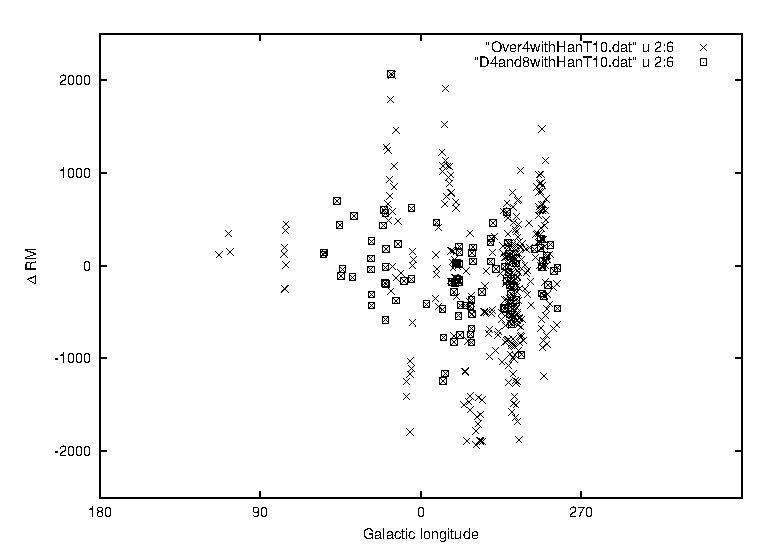
\includegraphics[width=8cm,clip]{pulsar/drm-l.eps}
\caption{パルサーペアから得た$\Delta RM$[rad/m$^2$]の銀経分布。$\times$は距離が4 kpc $<d<$ 12 kpcのパルサーからペアをとった場合、$\boxdot$は距離が4 kpc $<d<$ 8 kpcのパルサーからペアをとった場合。}
\label{drmlo}
\end{figure}

\begin{figure}[htb]
\centering
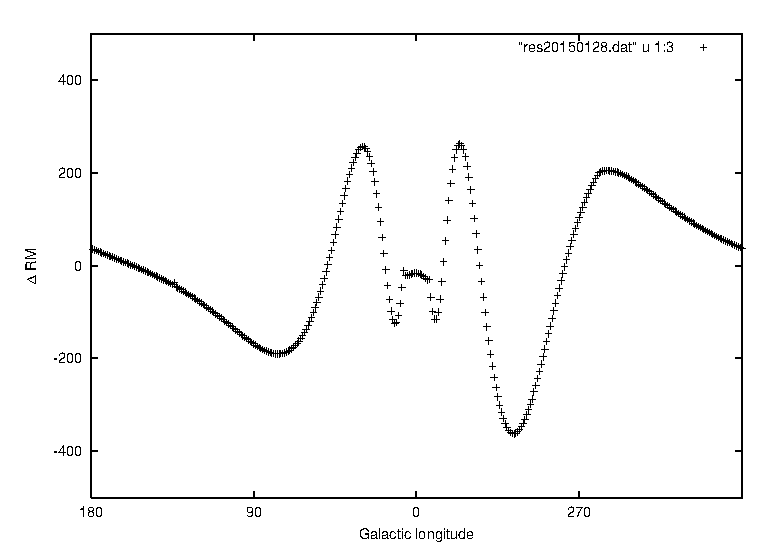
\includegraphics[width=8cm,clip]{pulsar/BSS-drml.eps}
\caption{銀河系に非軸対称な磁場モデルと電子密度を仮定した場合の$\Delta RM$の銀経分布}
\label{bssdrml}
\end{figure}

\begin{figure}[htb]
\centering
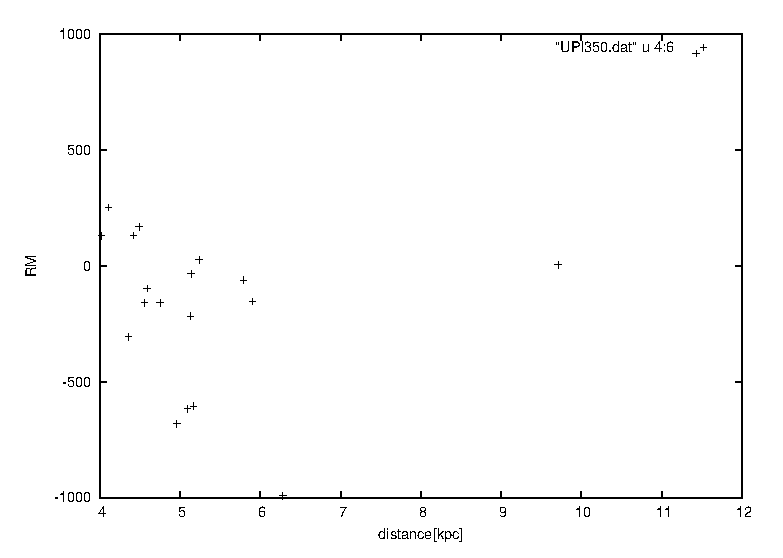
\includegraphics[width=8cm,clip]{pulsar/UPl350.eps}
\caption{$l \sim 350^{\circ}$のパルサーについて、$RM$と距離$d$の関係。}
\label{UPl350}
\end{figure}



\subsection{SKAとGiant Radio Pulses}

SKAでは、SKA-low, SKA-midを合わせると0.05-14GHzの広帯域化が実現される予定である。広帯域観測に基づくパルサーのGiant Radio Pulse研究の課題として、我々はパルス伝播路のプラズマ密度構造の探査の可能性に注目している。

パルサーでは、強磁場と高速自転のエネルギーにより、パルサー磁気圏から大量の(Crabパルサーで$\sim3\times10^{40}$個/秒)高エネルギー荷電粒子が放出されることが示唆されている。しかし現状では、パルサーの電磁場のエネルギーを荷電粒子のエネルギーにどう変換するか、つまり高エネルギー粒子をいかに生み出すか、そのメカニズムが解明されていない。我々はこの問題に迫るべく、まず、未だ解明されていないパルサー磁気圏、またその周囲における粒子の密度分布に迫ることを目指す。

我々は、広帯域のGRP同時観測により、周波数ごとのGRP到来時刻差の精密測定を行うことで、パルス伝播路、特にパルサー近傍のプラズマ密度構造に迫ろうとしている。電磁波はプラズマ中を伝播する際、低周波数ほど遅れて到来するという性質(``dispersion'')がある。周波数$f_1, f_2$を持つパルスの到来時刻差を$\Delta t$とすると\cite{LK04}、
\begin{equation}
\label{dispersion}
\Delta t = \int_{0}^{L}\frac{ds}{c\sqrt{1-\left(\frac{f_{p}}{f_{1}}\right)^{2}}} - \int_{0}^{L}\frac{ds}{c\sqrt{1-\left(\frac{f_{p}}{f_{2}}\right)^{2}}} 
\end{equation}
ここで、$f_p$はプラズマ振動数
\begin{equation}
\label{fpe}
f_{p} \equiv \sqrt{\frac{n_{e}q^{2}}{\pi m_{e}}} \sim 9\sqrt{n_{e}[\mathrm{cm}^{-3}]} [\mathrm{kHz}]
\end{equation}
であり、
$f_p \ll f_{1,2}$として展開すると、
\begin{equation}
\label{dispersion}
\Delta t\sim 4.15 \times 10^{-3} \mathrm{s} \left(f_{1,\mathrm{GHz}}^{-2}-f_{2,\mathrm{GHz}}^{-2}\right)DM_{\mathrm{pc/cm^{3}}}
+ 0.25 \times 10^{-12} \mathrm{s} \left(f_{1,\mathrm{GHz}}^{-4}-f_{2,\mathrm{GHz}}^{-4}\right)EM_{\mathrm{pc/cm^{6}}} 
\end{equation}
ここで、パルサーと観測者の間の距離をLとして、
\begin{equation}
DM\equiv \int_{0}^{L}n_{e} ds,  EM\equiv \int_{0}^{L}n_{e}^{2} ds
\end{equation}
と表される。$DM$は``Dispersion Measure''である。$EM$は制動放射における概念$[$例えば、\cite{Nakai08}など$]$を転用した``Emission Measure''である。

ところで、これまで多くの観測では、(\ref{dispersion})の第二項は小さいとして無視されてきた。しかし、もし視線上に局所的にプラズマ密度の高い領域が存在するならば、第二項は密度の2乗に比例するため、無視できなくなる場合がありうる。実際、CrabパルサーのGRPにおいて、第一項のみでは説明できない到来時刻差の検出が報告されており\cite{Ku08}、その原因としてCrab Nebula内の未知の高密度プラズマ領域によって生じた第二項の寄与の可能性が議論されている。従って、$EM$の測定による局所的な高密度領域の存在調査は、未解明であるパルサー磁気圏・パルサー風のプラズマ密度構造の理解につながりうる。

\cite{Ku08}は、44, 63, 111MHzの3帯域でのCrabパルサーGRPの同時観測により到来時刻差を測定し、 観測期間中の平均の$EM$の値として$\sim4\times10^{6}$pc/cm$^{6}$という結果を得た。パルサーの$DM$には時間的な変動がある\citep{Ly93}ので\footnote{``JODRELL BANK CRAB PULSAR MONTHLY EPHEMERIS'', \url{http://www.jb.man.ac.uk/~pulsar/crab.html}}、$EM$にも時間変動がありうるだろう。SKAを用いてさらに検証を行っていくことは重要である。

SKAを用いて広帯域の同時観測を行うことにより、より精度よく$DM$、$EM$を測定できることが期待される。具体的に、どの程度の$EM$の値まで検出することができるか?以下に、大雑把な見積もりを示す。式(\ref{dispersion})より、低周波数ほど$EM$の効果は顕著になると言えるから、SKAを用いた場合、まずSKA-midを用いて$DM$を決定し、その$DM$を用いてSKA-lowで観測されたGRPの到来時刻に$EM$の効果があるか否かを検証することになるだろう。

仮に、SKA-midにより$DM$を誤差$\delta DM$で決定したとする。SKA-lowの最低周波数($\equiv f_{\mathrm{min}}$)と最高周波数($\equiv f_{\mathrm{max}}$)のGRPの到来時刻差のうち、$DM$による寄与を除いてなお残る到来時刻差を$\Delta t'$とすると、式(\ref{dispersion})より、
\begin{eqnarray}
\label{delay}
\Delta t'&=& 0.25 \times 10^{-12} \mathrm{s} \left(f_{\mathrm{min},\mathrm{GHz}}^{-4}-f_{\mathrm{max},\mathrm{GHz}}^{-4}\right)EM_{\mathrm{pc/cm^{6}}} \\ \nonumber
&\pm& 4.15 \times 10^{-3} \mathrm{s} \left(f_{\mathrm{min},\mathrm{GHz}}^{-2}-f_{\mathrm{max},\mathrm{GHz}}^{-2}\right)\delta DM_{\mathrm{pc/cm^{3}}} 
\end{eqnarray}
となる\footnote{非一様なプラズマ中を伝播することによりパルスが鈍る効果$[$``scattering'', \cite{LK04}$]$は低周波数で顕著となるため、$\Delta t'$にはこれによる誤差が付きうる。しかし簡単のため、ここではその誤差を無視した。}。式(\ref{delay})から、
\begin{eqnarray}
EM_{\mathrm{pc/cm^{6}}}&=&\frac{\Delta t'}{0.25 \times 10^{-12} \left(f_{\mathrm{min},\mathrm{GHz}}^{-4}-f_{\mathrm{max},\mathrm{GHz}}^{-4}\right)} \\ \nonumber
&\pm&\frac{4.15 \times 10^{-3} \left(f_{\mathrm{min},\mathrm{GHz}}^{-2}-f_{\mathrm{max},\mathrm{GHz}}^{-2}\right)\delta DM_{\mathrm{pc/cm^{3}}}}{0.25 \times 10^{-12} \left(f_{\mathrm{min},\mathrm{GHz}}^{-4}-f_{\mathrm{max},\mathrm{GHz}}^{-4}\right)}
\end{eqnarray}
となる。第二項を評価することにより、検出可能な$EM$の最小値$EM_{\mathrm{min}}$を求めてみる。我々の1.4-2.2GHzでの観測の経験から、SKA-midを用いることにより、Crabパルサーについて$\delta DM\simeq0.001$pc/cm$^{3}$の精度で決定出来ると予想する。
一方、SKA-lowの現段階での$f_{\mathrm{min}}=0.05$GHz, $f_{\mathrm{max}}=0.30$GHzであるので、
\begin{equation}
EM_{\mathrm{min, SKA}}\simeq4.04\times10^{4} [\mathrm{pc/cm^{6}}]
\end{equation}
が検出可能な$EM$の最小値となる\footnote{ただし実際には、SKA-midの帯域にもわずかながら$EM$の効果がありうる。この効果を補正して$DM$決定をやり直し、また改めて$EM$を決める、というプロセスを収束するまで繰り返して$DM、EM$を決定すべきである。}。同様の見積もりをKuz'minらの観測に適用すると、
\begin{equation}
EM_{\mathrm{min, Kuz'min}}\simeq1.39\times10^{5} [\mathrm{pc/cm^{6}}]
\end{equation}
となる。従ってSKAによる観測の方が、Kuz'minらの観測で得られる30\%程度の大きさの$EM$まで決定できると言える。その他のGRPを放つパルサーでは$EM$の効果の検証はこれまで行われていないが、特にミリ秒パルサー$[$例えば\cite{So04, Bi14}など$]$ではintrinsicなGRPのdurationが短く、SKA-midを用いることでCrabパルサーと同程度の$DM$決定が期待できる。従って、上記のCrabパルサーでの見積もりと同程度の$EM$の検出が期待できる。

GRPは通常のパルスと比べS/N比も大きく、積分の必要もないため、GRP発生時毎に$DM$、$EM$を決定できる。これにより、数分・数時間での$DM$、$EM$の変動が調査可能であり、変動の存在が確かめられれば、それは高密度プラズマ領域のサイズに対する制限となりうる。加えて、領域のプラズマ密度が大きくなると、プラズマ周波数$f_{p}$が観測周波数$f$に近づく。すると、$f$における電磁波の群速度は0に近づく。従って、$EM$でも説明できないずれ、さらには低周波数でスペクトルに「カットオフ」が見られるかもしれない。

このように、0.05-14GHzまでの広帯域観測が可能となる予定のSKAでは、パルサー近傍のプラズマ密度構造にこれまで以上に迫ることが期待できる。それらとパルサーの年齢、spin-down 光度(自転エネルギー損失率)などの性質の間に相関が見られないか、など興味は尽きない。


